\chapter{Método do trabalho} \label{cap:metodo}

O presente capítulo discute três ideias de arquitetura para o sistema proposto, com o objetivo de identificar alternativas viáveis para equilibrar segurança, privacidade e custo operacional no contexto de monitoramento veicular. Em vez de apresentar uma implementação final, o foco está na formulação e análise comparativa das abordagens candidatas, destacando seus pressupostos, vantagens, limitações e requisitos técnicos.


\section{Arquitetura com BOLO e desbloqueio excepcional por quórum}
Esta arquitetura parte de duas premissas de projeto: (i) o sistema não pode impedir o uso operacional das câmeras para consultas do tipo \textit{Be On the Lookout} (BOLO), como comparação com bases de veículos roubados, mandados de busca e casos de \textit{Amber Alert}; e (ii) o mesmo sistema deve dificultar tecnicamente a vigilância em massa da população. Para atender a essas premissas, o modelo separa o fluxo de resposta imediata do fluxo de acesso investigativo retrospectivo.

\begin{figure}[htbp]
    \centering
    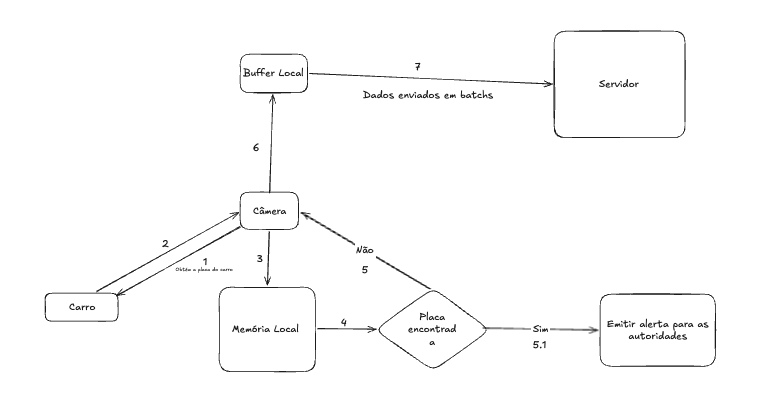
\includegraphics[width=0.9\textwidth]{Imagens/Cap3/Proposta_Modelo_BOLO.png}
    \caption{Desenho da arquitetura proposta com fluxo BOLO e desbloqueio excepcional por quórum.}
    \label{fig:arquitetura-bolo-quorum}
\end{figure}

No fluxo BOLO, a verificação ocorre de forma direcionada e orientada por lista de interesse previamente definida, permitindo alertas em tempo quase real quando houver correspondência com alvos específicos. No fluxo de armazenamento, cada câmera possui um identificador único no banco de dados e registra, para cada captura, a placa em formato criptografado, o horário do evento e metadados veiculares relevantes. Essa estrutura permite rastreabilidade por origem e por janela temporal, sem expor diretamente o conteúdo em texto claro.

Como mecanismo de contenção institucional para acessos amplos, a arquitetura prevê uma chave mestre fracionada entre oito representantes (deputados estaduais), em esquema de compartilhamento de segredo, onde metade deve se juntar para obter a chave. Assim, somente a reunião de pelo menos quatro partes autorizadas permite reconstruir a chave de exceção para abrir informações de múltiplas câmeras em um período de interesse. Portanto, acessos extraordinários deixam de depender de decisão unilateral e passam a exigir coordenação política explícita, aumentando auditabilidade e custo institucional de consultas massivas.

Em síntese, a proposta busca preservar a efetividade do BOLO para casos urgentes e específicos, enquanto impõe barreiras técnicas e de governança contra uso indiscriminado da base histórica. 

\section{Arquitetura de Vigilância Criptografada com Governança por Quórum e Desbloqueio de Exceção.}
A arquitetura proposta organiza-se como um ecossistema de custódia de dados fundamentado no princípio da segurança em múltiplas camadas, estruturando-se em quatro eixos fundamentais: captura e proteção na borda, custódia cega, governança de acesso e mecanismos de exceção. O design tem como objetivo primordial garantir a privacidade dos cidadãos através de um custo computacional linear por registro decodificado e de uma rastreabilidade institucional perene, alinhando-se tecnicamente à tese das Crypto Crumple Zones e ao princípio jurídico da proporcionalidade nas quebras de sigilo.

\begin{figure}[htbp]
    \centering
    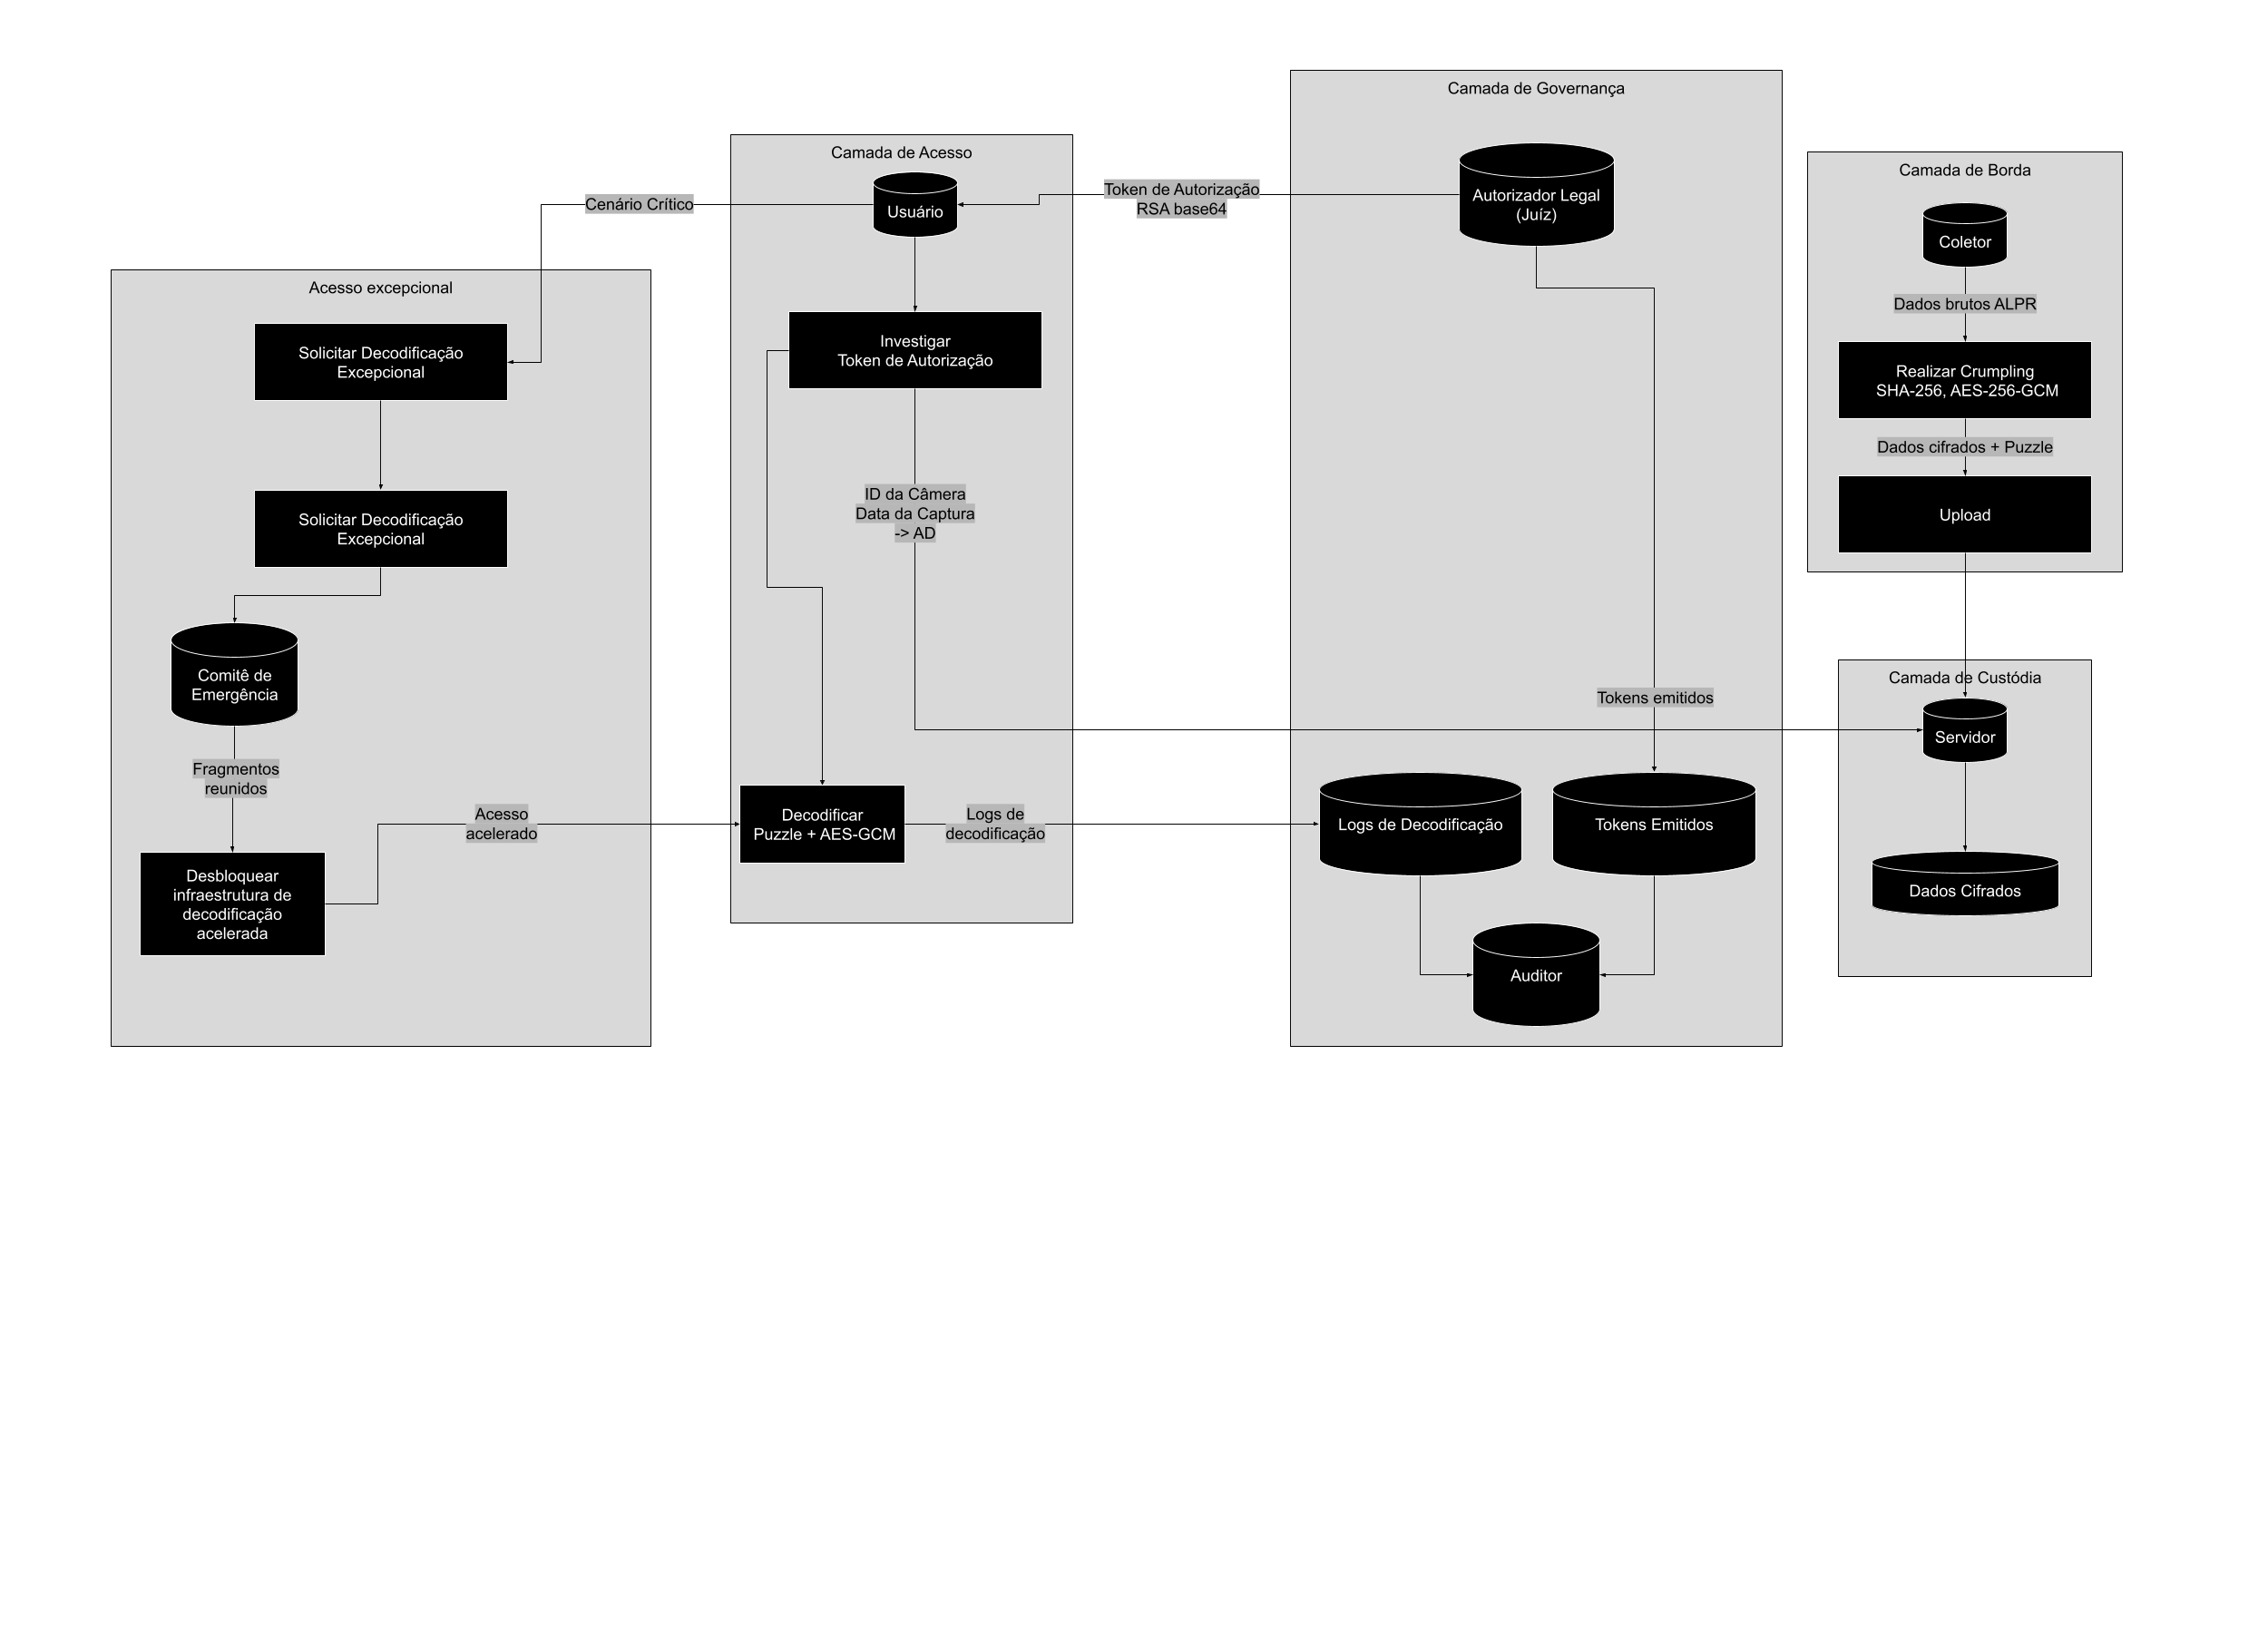
\includegraphics[width=0.9\textwidth]{Imagens/Cap3/Arquitetura de Vigilância Criptografada com Governança por Quórum e Desbloqueio de Exceção.png}
    \caption{Fluxograma da Arquitetura de Vigilância Criptografada, destacando a separação entre a captura de dados na borda, a custódia segura e o modelo de governança baseado em autorização judicial e quórum político para acessos de exceção.}
    \label{fig:arquitetura-bolo-quorum}
\end{figure}

O ciclo de vida do dado inicia-se na Camada de Borda, especificamente no coletor ALPR, onde a privacidade é assegurada pelo método de Crumpling. Neste estágio, os dados brutos são transformados em estruturas criptográficas complexas antes de qualquer transmissão para a rede. Para cada captura — que compreende a placa, localização, timestamp e identificador da câmara — o coletor gera uma chave mestra aleatória $k_0$ de 256 bits e deriva uma chave de cifragem secundária $k_{ccz}$ via SHA-256. O payload, contendo informações sensíveis como latitude e longitude, é cifrado utilizando o algoritmo AES-256-GCM. Este protocolo é reforçado pelo uso de Associated Data (AD), que vincula o cifrado ao contexto específico da captura, garantindo que qualquer alteração no ciphertext ou no identificador da câmara invalide a decifragem. Complementarmente, o sistema gera um "puzzle" criptográfico ao revelar apenas uma fração de $k_0$, mantendo uma entropia oculta de $l$ bits. Este puzzle atua como uma barreira de latência deliberada, exigindo prova de trabalho para a recuperação da chave e impedindo tecnicamente a decodificação em massa não autorizada. Após o envio do pacote cifrado, o texto claro da placa e a chave $k_0$ completa são permanentemente descartados na borda.

Na sequência, os pacotes são transmitidos para a Camada de Custódia, onde o servidor central atua como um repositório cego. Nesta fase, os dados permanecem em repouso estritamente cifrados, e o servidor, embora responsável pelo armazenamento, não possui as chaves necessárias para a leitura do conteúdo. A indexação é realizada exclusivamente por metadados não sensíveis, permitindo a localização temporal e geográfica de eventos sem expor a identidade dos alvos, sendo que a liberação de qualquer conteúdo condicional à apresentação de um token de autorização válido.

A Camada de Governança e a Camada de Acesso medeiam o fluxo de informação. A decodificação de um registro exige a intervenção de um Autorizador Legal (Magistrado), que emite um token de autorização baseado em criptografia assimétrica RSA. O servidor utiliza a chave pública para verificar a assinatura digital em base64 e o vínculo do token com os dados solicitados. Este mecanismo é estritamente granular, restringindo o acesso apenas ao escopo autorizado. Para garantir a conformidade e coibir abusos, um Auditor realiza a reconciliação contínua entre os tokens emitidos e os logs de decodificação, estabelecendo uma trilha de auditoria que permite verificar se o volume de dados processados corresponde estritamente às ordens judiciais expedidas.

Por fim, para mitigar o risco de vigilância em massa ou abusos unilaterais, a arquitetura implementa um Mecanismo de Exceção gerido por um Comitê de Emergência. Em cenários críticos, o acesso à infraestrutura de decodificação acelerada — necessária para resolver grandes volumes de puzzles em tempo útil — depende da reconstrução de uma chave mestra fragmentada via esquemas de segredo compartilhado. O desbloqueio do sistema só ocorre quando um quórum predefinido de representantes reúne os seus fragmentos. Esta abordagem transmuta uma limitação técnica numa salvaguarda política de alto nível, garantindo que qualquer tentativa de vigilância em larga escala exija coordenação institucional e deixe rastros administrativos e políticos indeléveis.

\section{Arquitetura com Treshold Criptográfico}
A robustez deste modelo de governança reside na imposição de barreiras multi-camadas para o acesso aos dados, diferenciando o uso rotineiro da análise de exceção. Para o Acesso Comum, a arquitetura estabelece um limiar técnico-administrativo: a liberação de dados depende da apresentação de um Token de Autorização emitido pelo Judiciário, somado obrigatoriamente a uma Prova de Trabalho (\textit{Proof-of-Work} - PoW) realizada pela infraestrutura da Polícia. Esse requisito de gasto computacional atua como um desincentivo econômico e técnico contra varreduras massivas e consultas automatizadas sem alvo definido.

\begin{figure}[H]
    \centering
    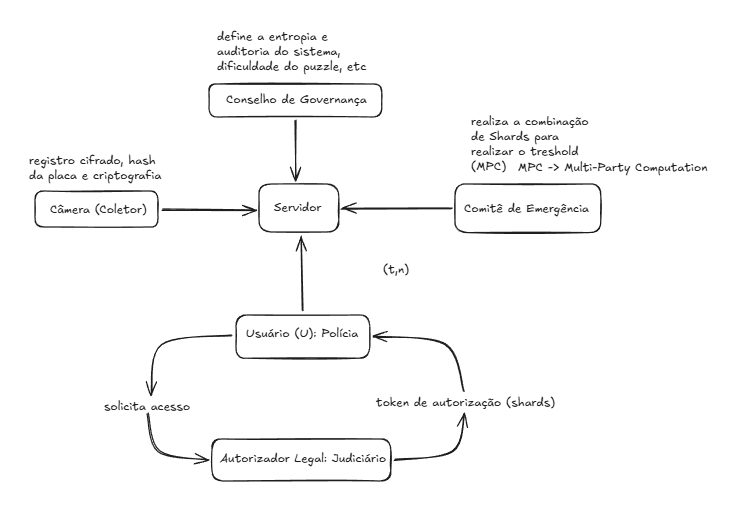
\includegraphics[width=0.8\textwidth]{Imagens/Cap3/Arquitetura Treshold Inicial.png}
    \caption{Desenho da arquitetura proposta com treshold criptográfico.}
    \label{fig:arquitetura-bolo-quorum}
\end{figure}

Para cenários de Acesso Excepcional, onde a urgência ou a sensibilidade superam os trâmites do fluxo comum, a arquitetura introduz um Comitê de Emergência. Neste nível, a chave de acesso é fragmentada em \textit{shards} distribuídos entre os membros do comitê via \textit{Multi-Party Computation} (MPC). A reconstrução da autorização exige que um quórum mínimo (limiar) de membros forneça suas partes, garantindo que nenhum agente isolado, nem mesmo o administrador do sistema, possua controle total sobre a base histórica de placas (ALPR).

Sob a supervisão de um Conselho de Governança, os parâmetros de esforço da PoW e os valores de limiar do comitê são calibrados e auditados periodicamente. Dessa forma, o projeto não apenas protege os dados através de criptografia, mas submete o acesso a um rastro de auditoria duplo: a necessidade de autorização externa e o custo computacional explícito, elevando o custo institucional de qualquer tentativa de vigilância indiscriminada.

Entretanto, a análise dessa arquitetura revelou uma vulnerabilidade persistente no estágio de execução do acesso excepcional: o risco de exposição da chave no momento da reconstrução. Ao exigir que os membros do comitê forneçam seus shards para a montagem do segredo dentro do ambiente computacional do solicitante, a chave mestra torna-se temporariamente visível e, portanto, tecnicamente comprometida para usos futuros. Essa fragilidade compromete a segurança do sistema, uma vez que a posse da chave reconstruída permitiria à entidade policial realizar consultas retroativas ou futuras sem a necessidade de uma nova convocação do quórum. Consequentemente, o modelo atual impõe um alto custo operacional de manutenção, exigindo que todo o conjunto de fragmentos seja resetado e redistribuído após cada ativação do fluxo de emergência para restauro de integridade.